\chapter{Resultados}

\section{VQ-VAE base}

\subsection{Calidad de reconstrucción}

El VQ-VAE base fue entrenado durante 16 epochs sobre 718.673 imágenes 2grid 
del dataset ELAsTiCC-1. Al término del entrenamiento, la pérdida total sobre 
el conjunto de entrenamiento alcanzó 0.0003, con una pérdida de 
reconstrucción de 0.000216. La perplexity efectiva del codebook se situó en 
$\sim$162 durante el entrenamiento y $\sim$196 sobre el conjunto de 
validación, lo que indica que entre 162 y 196 de los 512 embeddings 
disponibles participan activamente en la representación del dataset 
(Tabla~\ref{tab:vqvae_base_results}).

\begin{table}[H]
\centering
\begin{tabular}{|l|c|}
\hline
\textbf{Métrica} & \textbf{Valor} \\
\hline
train/loss (mejor checkpoint) & 0.0003 \\
train/recon\_loss              & 0.000216 \\
train/perplexity               & $\sim$162 \\
val/perplexity                 & $\sim$196 \\
\hline
\end{tabular}
\caption{Resultados del VQ-VAE base al finalizar el entrenamiento.}
\label{tab:vqvae_base_results}
\end{table}


\subsection{Análisis del espacio latente discreto}
\label{sec:umap_base}

Para caracterizar la organización interna del espacio latente aprendido, se 
proyectaron los tokens generados sobre una muestra del conjunto de validación 
mediante UMAP, asignando a cada punto el color correspondiente al tipo de 
supernova de la imagen de origen. La Figura~\ref{fig:umap_tokens} presenta el 
resultado.

\begin{figure}[H]
\centering
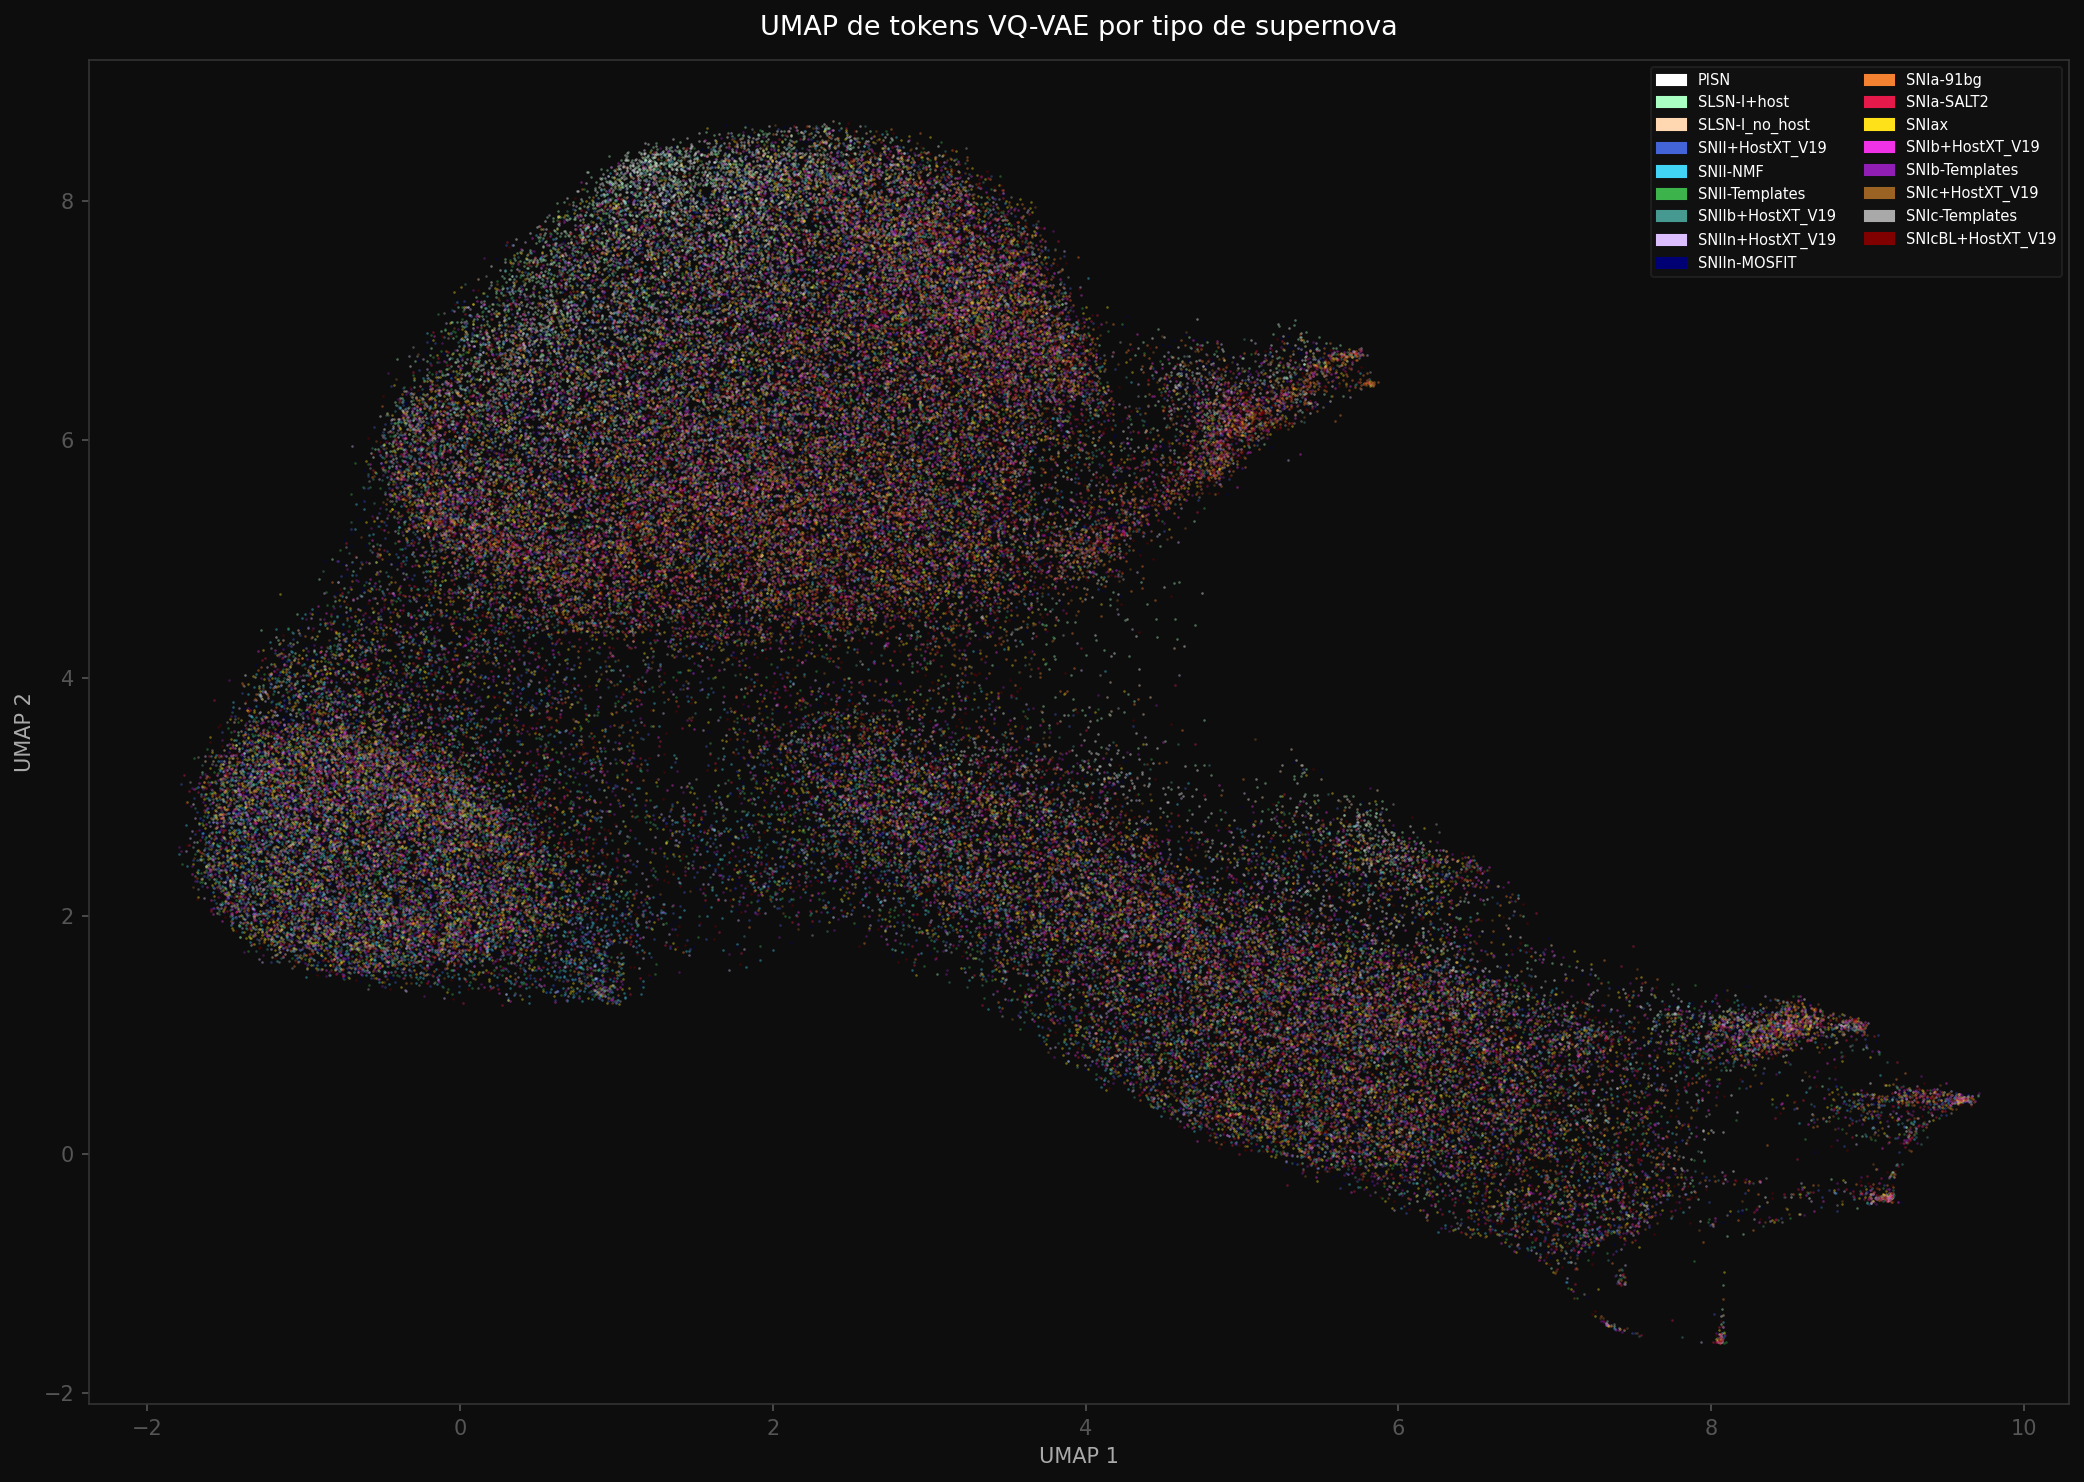
\includegraphics[width=\textwidth]{img/umap_tokens.png}
\caption{UMAP de tokens del VQ-VAE base coloreados por tipo de supernova. 
Cada punto corresponde a un token generado por una imagen 2grid del conjunto 
de validación.}
\label{fig:umap_tokens}
\end{figure}

La proyección revela una estructura geométrica con masa central compacta y 
varios brazos periféricos. Los 17 tipos de supernovas se distribuyen de forma 
mezclada a lo largo de toda la estructura, sin formar clusters diferenciados 
por clase. Para cuantificar esta distribución, se identificaron cinco regiones 
geográficas en el UMAP y se calculó la composición de tipos dentro de cada 
una (Figura~\ref{fig:umap_zoom} y Figura~\ref{fig:umap_pies}).

\begin{figure}[H]
\centering
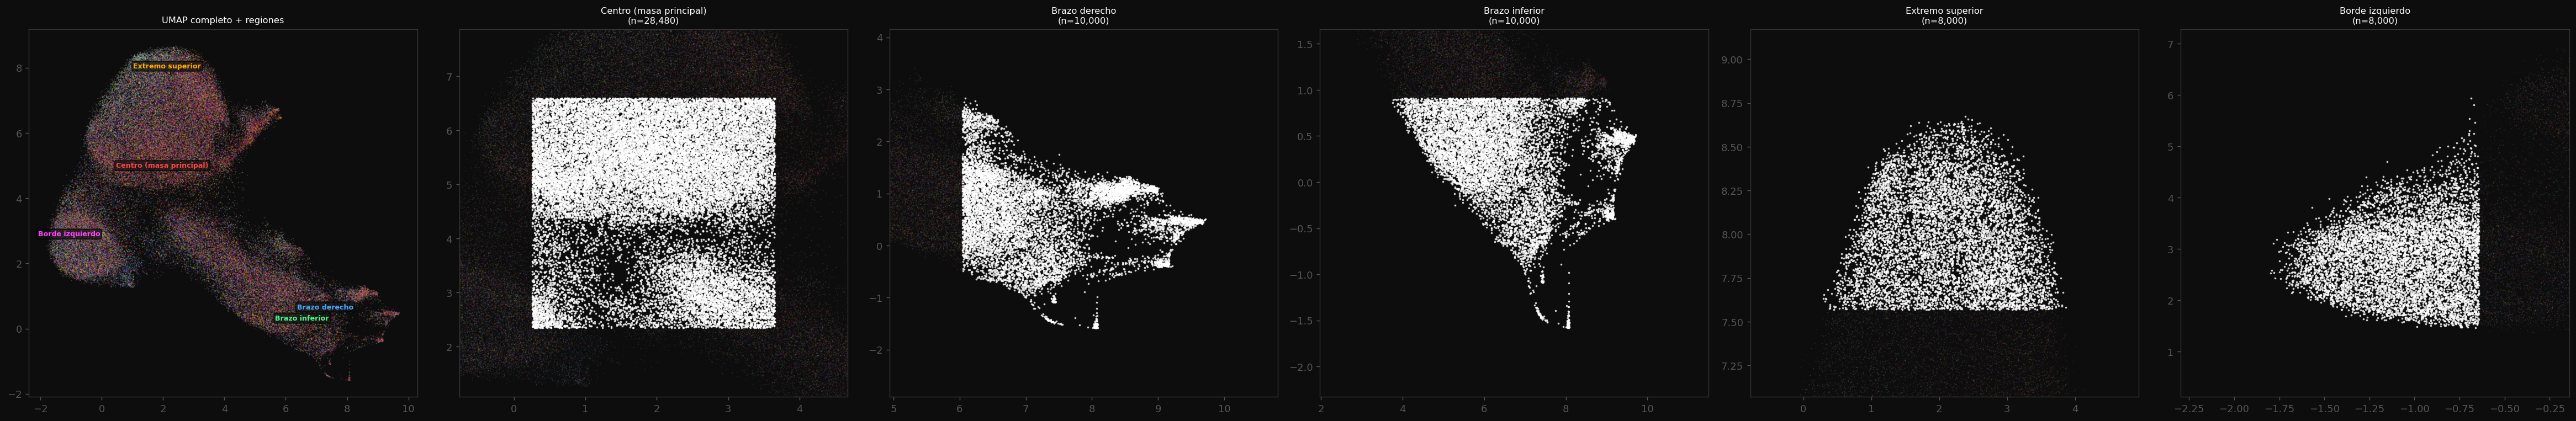
\includegraphics[width=\textwidth]{img/umap_zoom_regions.png}
\caption{Delimitación de las cinco regiones identificadas en el espacio UMAP: 
masa central, brazo derecho, brazo inferior, extremo superior y borde 
izquierdo.}
\label{fig:umap_zoom}
\end{figure}

\begin{figure}[H]
\centering
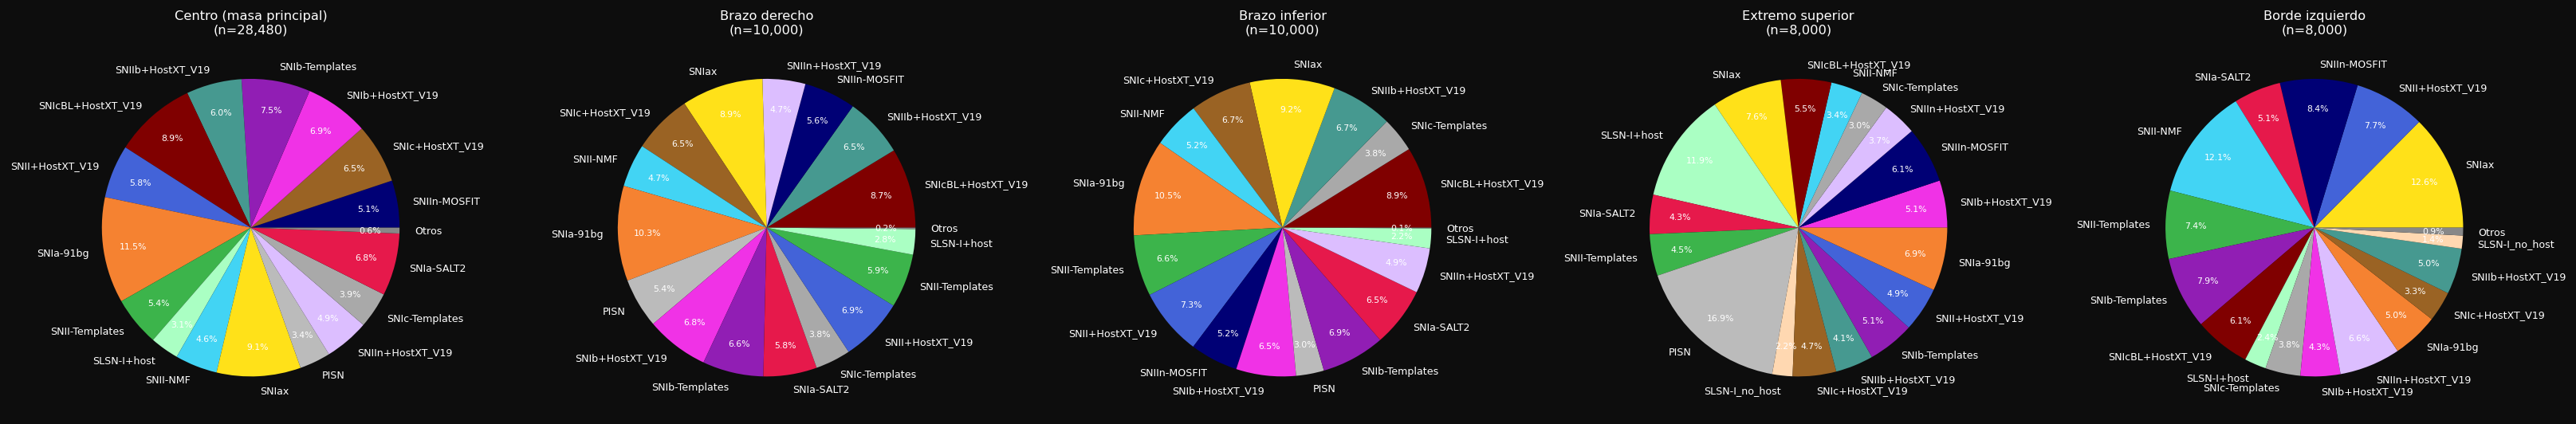
\includegraphics[width=\textwidth]{img/umap_composition_pies.png}
\caption{Composición por tipo de supernova en cada región del UMAP. La 
distribución de clases es similar entre zonas, sin dominancia de ningún tipo 
particular.}
\label{fig:umap_pies}
\end{figure}

Ninguna región está dominada por un tipo particular y la mezcla de clases es 
similar entre zonas, con variaciones menores que se explican por el desbalance 
del dataset. La Figura~\ref{fig:umap_examples} muestra imágenes 2grid 
representativas de cada región: las curvas de luz varían morfológicamente 
(el brazo derecho agrupa curvas con peaks más estrechos y la masa central 
concentra morfologías más extendidas), pero esa variación no coincide con 
los límites entre tipos astronómicos.

\begin{figure}[H]
\centering
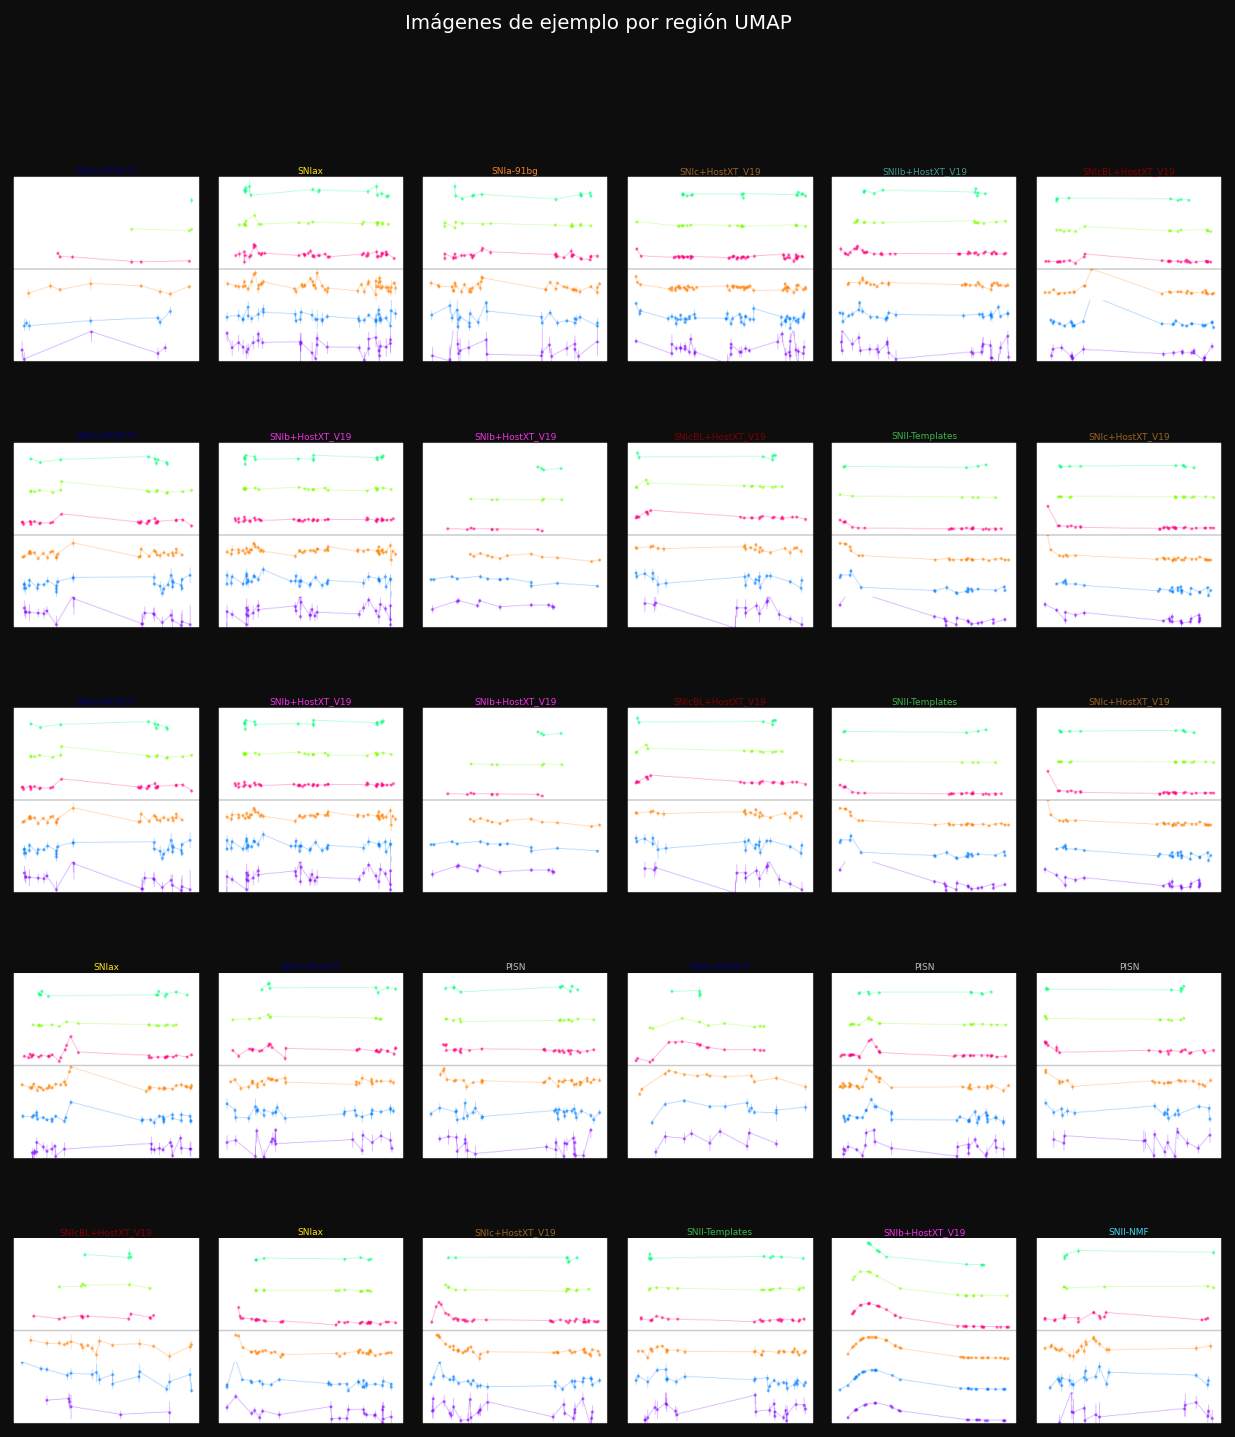
\includegraphics[width=\textwidth]{img/umap_example_images.png}
\caption{Imágenes 2grid de ejemplo por región del UMAP. Los títulos en color 
indican el tipo de supernova de cada imagen.}
\label{fig:umap_examples}
\end{figure}

El VQ-VAE base organiza el espacio latente por morfología visual de la curva 
de luz, no por tipo de objeto. La clasificación por tipo requiere una señal 
supervisada explícita, lo que justifica la extensión descrita en la sección 
siguiente.

\section{VQ-VAE con clasificación supervisada}
\label{sec:cls_supervisada}

\subsection{Entrenamiento}

El VQ-VAE extendido con un módulo de clasificación supervisada 
(\textit{classification head}) sobre $\mathbf{z}_q$ se entrenó sobre el mismo 
conjunto de 718.673 imágenes, incorporando la pérdida de clasificación con 
peso $\lambda = 0.1$. El modelo converge en 7 epochs, alcanzando una 
exactitud de validación de 55.6\% y una pérdida total de 0.1188 en el mejor 
checkpoint. La exactitud sobre el conjunto completo de validación (109.737 
imágenes) es 38.8\%, reflejo del desbalance entre tipos: la matriz de 
confusión muestra un recall de 0.88 para PISN y 0.81 para SLSN-I+host, 
mientras SNIIb y SNIc-Templates no superan 0.02 
(Figura~\ref{fig:confusion_matrix}).

\begin{figure}[H]
\centering
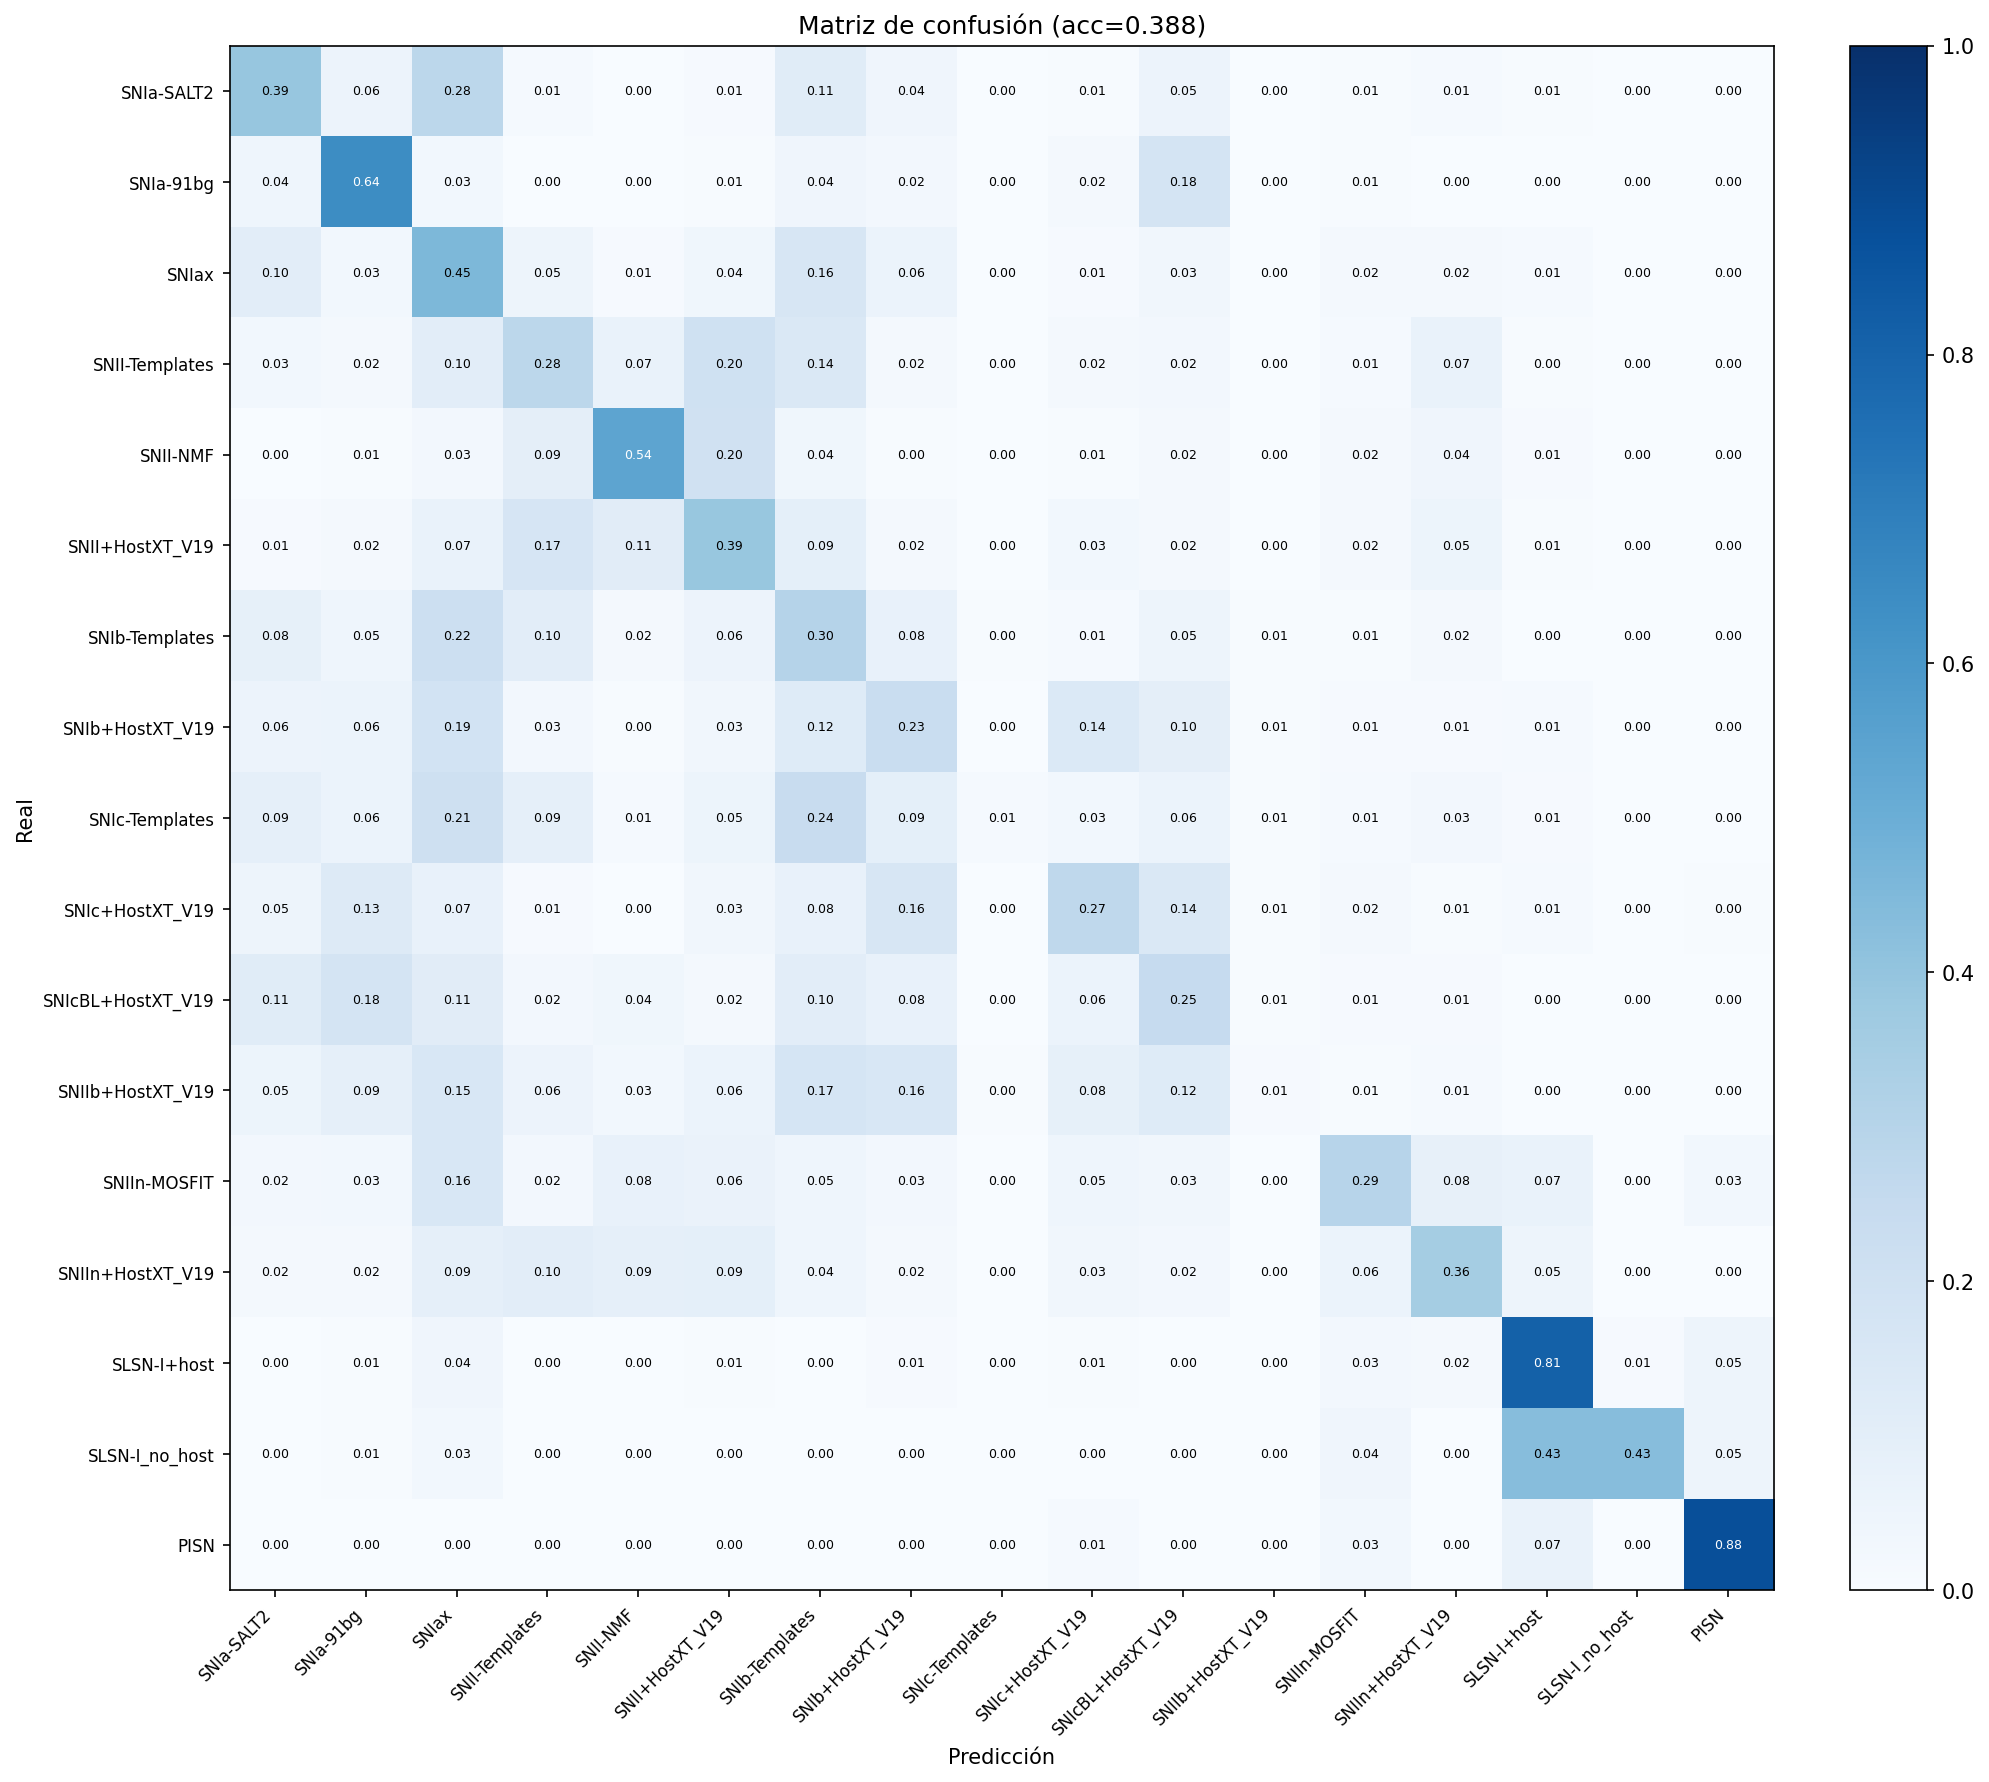
\includegraphics[width=\textwidth]{img/confusion_matrix.png}
\caption{Matriz de confusión del módulo de clasificación supervisada sobre el 
conjunto de validación (109.737 imágenes, 17 clases). Las filas corresponden 
a la clase verdadera y las columnas a la clase predicha. PISN y SLSN-I+host 
concentran la mayor exactitud por clase; los tipos morfológicamente similares 
entre sí (SNIIb, SNIc-Templates) presentan la mayor tasa de confusión.}
\label{fig:confusion_matrix}
\end{figure}

Buena parte de esa confusión ocurre entre subtipos que comparten morfología, por lo que la exactitud sobre las 17 clases subestima lo que el clasificador efectivamente distingue. Agrupando los tipos en seis categorías astronómicas se obtiene un F1 macro de 0.64 y un F1 ponderado de 0.58, según se muestra en la Figura~\ref{fig:confusion_matrix_grouped} y se detalla en la Tabla~\ref{tab:cls_grouped_metrics}.

\begin{figure}[H]
\centering
\insertimage[\label{fig:confusion_matrix_grouped}]{img/confusion_matrix_grouped.png}{width=0.75\textwidth}{Matriz de confusión agrupada en seis categorías astronómicas. Los valores corresponden al recall por grupo, es decir la fracción de objetos reales de cada categoría clasificados correctamente.}
\end{figure}

\begin{table}[H]
\centering
\begin{tabular}{|l|c|c|c|c|}
\hline
\textbf{Grupo} & \textbf{Precisión} & \textbf{Recall} & \textbf{F1} & \textbf{N} \\
\hline
SNIa  & 0.51 & 0.67 & 0.58 & 27.224 \\
SNIbc & 0.54 & 0.52 & 0.53 & 33.885 \\
SNII  & 0.65 & 0.56 & 0.60 & 25.840 \\
SNIIn & 0.58 & 0.39 & 0.47 & 11.796 \\
SLSN  & 0.73 & 0.83 & 0.78 &  5.502 \\
PISN  & 0.90 & 0.88 & 0.89 &  5.490 \\
\hline
\textbf{Promedio macro}     & 0.65 & 0.64 & 0.64 & 109.737 \\
\textbf{Promedio ponderado} & 0.59 & 0.59 & 0.58 & 109.737 \\
\hline
\end{tabular}
\caption{Métricas de clasificación por grupo sobre el conjunto de validación agrupado en seis categorías, donde N es el número de muestras de cada grupo.}
\label{tab:cls_grouped_metrics}
\end{table}

El patrón es consistente con la organización del codebook descrita más adelante, ya que PISN y SLSN, que son los tipos físicamente más distintos del resto, obtienen los F1 más altos con 0.89 y 0.78, mientras que SNIIn resulta el más difícil con 0.47 por su confusión frecuente con SNII, y SNIa, SNIbc y SNII quedan en un rango intermedio de entre 0.53 y 0.60.

\subsection{Análisis del codebook con señal supervisada}

Con 512 embeddings activos sobre 512 totales, el codebook se utiliza por 
completo, a diferencia del modelo base donde la perplexity efectiva era de 
$\sim$162--196. La pureza media del codebook es 0.154: con 17 clases, la 
pureza aleatoria esperada sería $1/17 \approx 0.059$, de modo que los 
embeddings aprendidos son $\sim$2.6 veces más puros que el azar, sin llegar 
a una especialización fuerte.

La Figura~\ref{fig:umap_codebook_cls} presenta la proyección UMAP de los 512 
embeddings del codebook, coloreada por clase dominante (izquierda) y por 
pureza (derecha).

\begin{figure}[H]
\centering
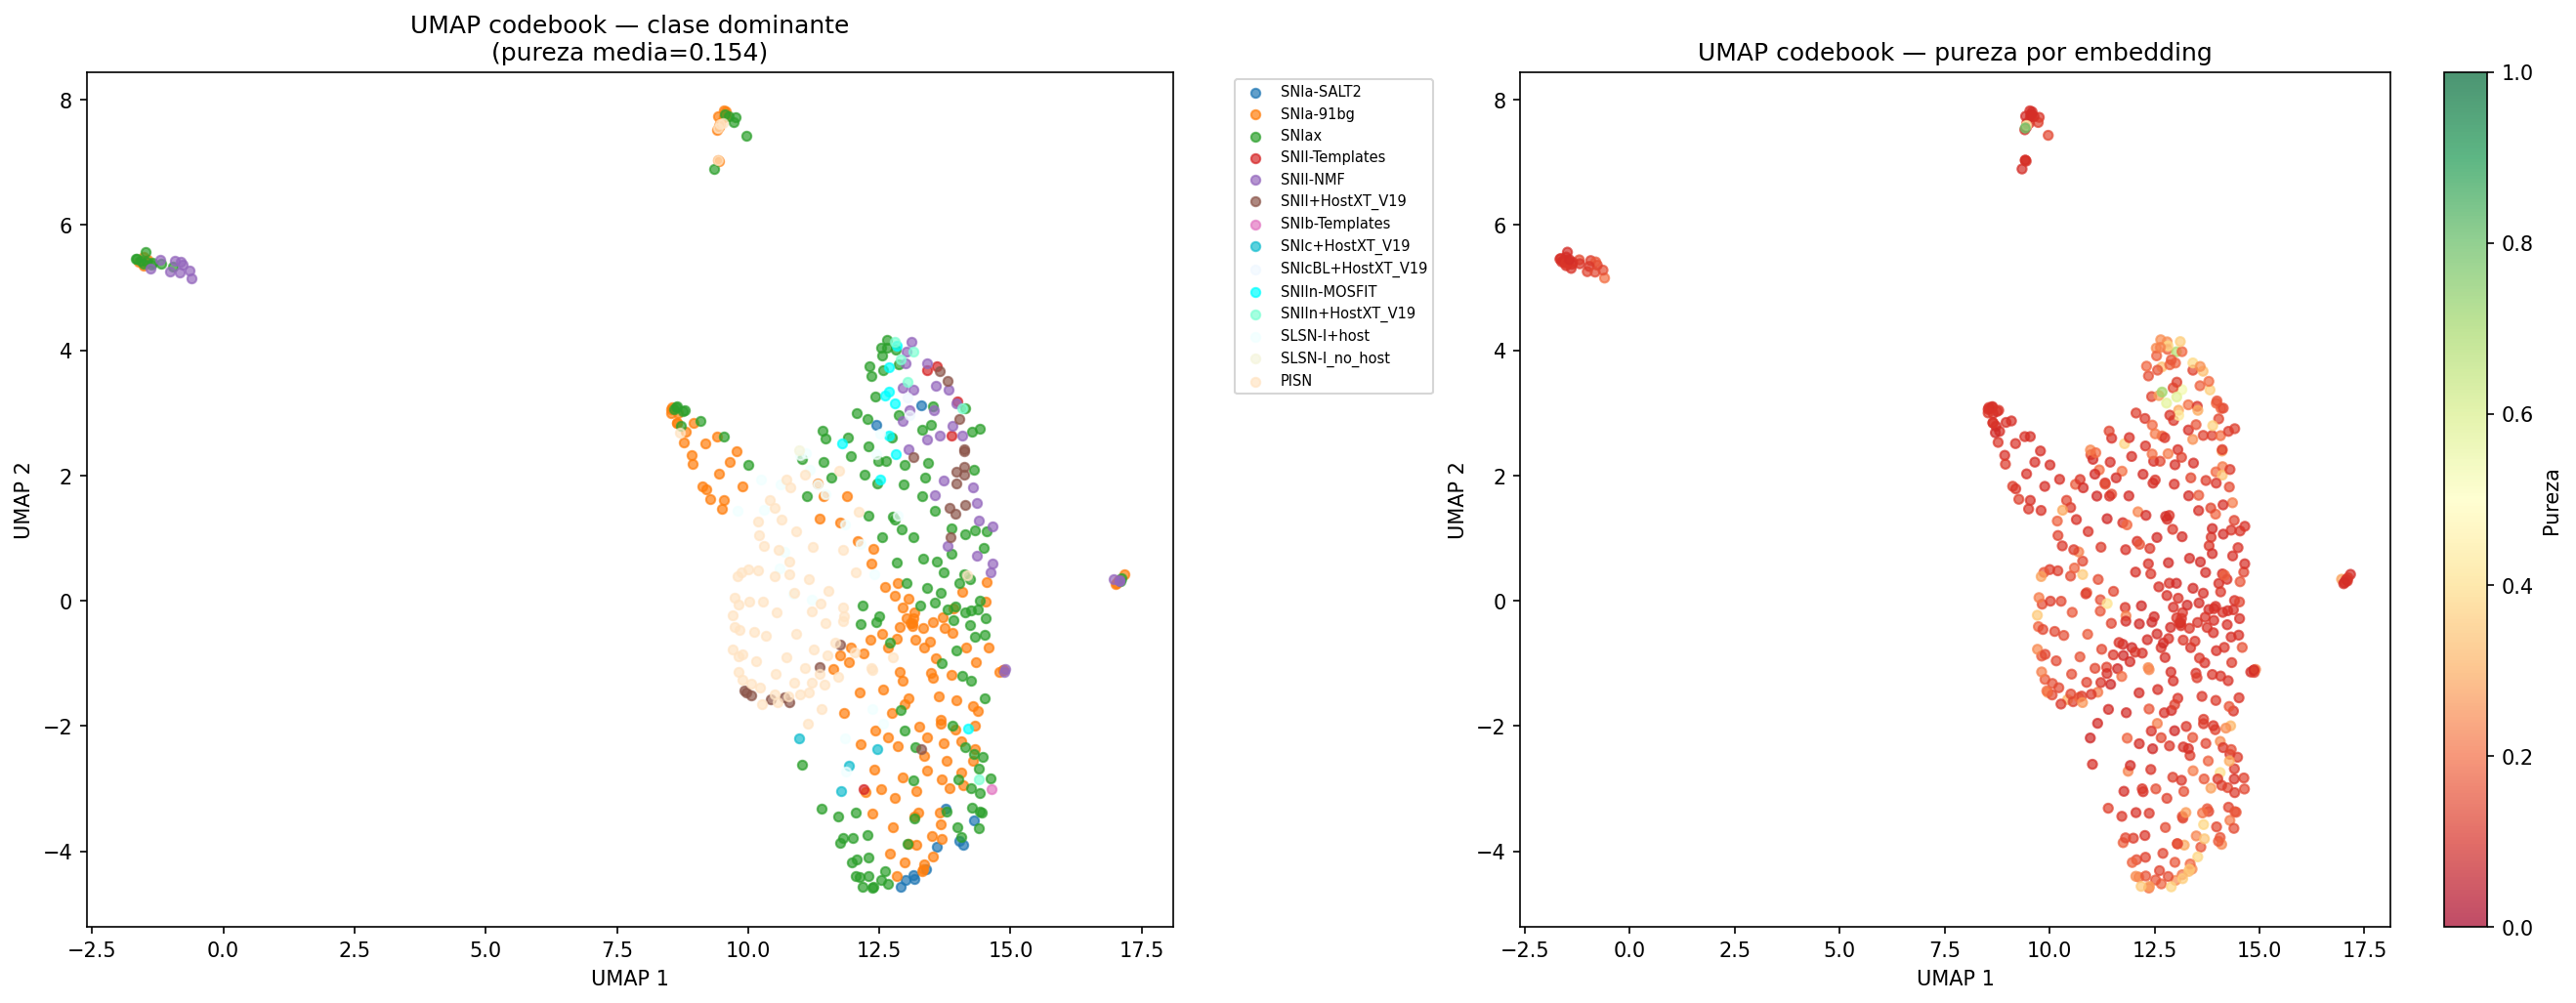
\includegraphics[width=\textwidth]{img/umap_codebook_cls.png}
\caption{UMAP de los 512 embeddings del codebook tras el entrenamiento con 
clasificación supervisada ($\lambda = 0.1$). Izquierda: color por clase 
dominante de cada embedding. Derecha: color por pureza 
($\text{pureza}(k) = \text{count}(k,\,c^*) / \sum_c \text{count}(k,c)$). 
Pureza media: 0.154.}
\label{fig:umap_codebook_cls}
\end{figure}

La estructura del UMAP revela dos comportamientos distintos. El cluster 
principal agrupa la mayoría de los embeddings con pureza baja (0.1--0.3), 
donde los tipos de SN estándar (SNIa, SNII, SNIb, SNIc) coexisten sin 
separación clara. Fuera de este cluster principal aparecen dos grupos 
aislados de alta pureza ($\geq 0.8$): uno dominado por SLSN-I y otro por 
PISN. Estos dos tipos son los morfológicamente más distintos del resto del 
dataset, con curvas de mayor duración y brillo, y son precisamente los que el 
módulo de clasificación identifica con mayor recall (0.81 y 0.88 
respectivamente).

\subsection{Comparación con el modelo base}

El VQ-VAE base organiza el espacio latente por morfología visual de la curva 
de luz, sin correspondencia con los tipos astronómicos 
(Sección~\ref{sec:umap_base}). La señal supervisada desplaza parcialmente 
esa organización: los tipos más atípicos quedan aislados en embeddings 
dedicados de alta pureza, mientras los tipos estándar, cuyas curvas de luz 
son morfológicamente similares entre sí, permanecen mezclados.

Este resultado es consistente con la exactitud diferencial del módulo de 
clasificación: $\lambda = 0.1$ alcanza para separar PISN y SLSN-I, pero no 
para discriminar tipos con morfologías parecidas como SNIIb y SNIc. La 
organización semántica del codebook refleja directamente la dificultad 
intrínseca del problema de clasificación sobre representaciones visuales de 
curvas de luz.

\section{Codificación del flujo}
\label{sec:res_codificacion}

\subsection{Saturación de la codificación lineal}

El reescalado lineal entre percentiles de la Ecuación~\ref{eq:enc_lineal} pierde sensibilidad justo en el régimen de anomalías grandes. Inyectando el pico de la Ecuación~\ref{eq:inyeccion} y midiendo cómo reaccionan los estadísticos de escala del propio objeto, $Q_{0.99}$ se multiplica por 60 entre $\Delta f = 10$ y $\Delta f = 1000$, mientras el MAD crece apenas 1.4 veces, por lo que es el propio outlier el que termina arrastrando la escala con la que debería medirse.

El efecto sobre la imagen es directo: con la escala congelada al valor del control, las imágenes de $\Delta f = 20$, 50, 100 y 200 resultan idénticas píxel a píxel, ya que el pico queda fuera del carril y el recorte lo deja apoyado en el borde superior. Sin congelar la escala, la fracción de píxeles que difieren del control pasa de 12.58\% en $\Delta f = 30$ a 13.02\% en $\Delta f = 100$, de modo que triplicar la amplitud alcanza a cambiar solo el 0.44\% de la imagen.

\begin{figure}[H]
\centering
\insertimage[\label{fig:saturacion}]{img/saturacion_imagen.png}{width=\textwidth}{Saturación de la codificación lineal, medida como porcentaje de píxeles que difieren del control. Izquierda: con escala libre, el cambio en la imagen se estanca cerca del 13\% a partir de $\Delta f = 40$ y el recall del detector deja de crecer con él. Derecha: con la escala congelada al control, el recorte lleva el pico al borde del carril y 105 de 280 pares de niveles vecinos producen imágenes idénticas.}
\end{figure}

Verificando lo mismo un nivel más abajo, sobre el mapa de tokens que efectivamente recibe el prior, el 95\% de los tokens sí cambia respecto del control. La representación no se congela, pero cambia de una manera que el prior sigue considerando normal: la curva completa se reescaló, y una curva reescalada es una curva plausible. La normalización por objeto resulta contraproducente para detectar outliers precisamente porque el outlier redefine su propia escala.

\subsection{Comparación entre codificaciones}

Las tres codificaciones se compararon en igualdad de condiciones, entrenando para cada una un VQ-VAE y un prior MaskGIT propios sobre el mismo subconjunto de 196.000 imágenes, con idénticos hiperparámetros y particiones. La evaluación usa 39 SNIa, tras excluir un objeto presente en el conjunto de entrenamiento del subconjunto.

\begin{table}[H]
\centering
\begin{tabular}{|l|c|c|c|c|c|c|}
\hline
\textbf{Codificación} & \multicolumn{5}{c|}{\textbf{Recall por} $\Delta f$} & \textbf{Monotonía} \\
\cline{2-6}
 & 10 & 50 & 100 & 300 & 500 & (Spearman) \\
\hline
Lineal (Ec.~\ref{eq:enc_lineal}) & 0.10 & 0.41 & 0.33 & 0.23 & 0.38 & $+0.09$ \\
\texttt{mad100}                  & 0.05 & 0.36 & 0.39 & 0.10 & 0.08 & $+0.16$ \\
\texttt{mad300}                  & \textbf{0.31} & \textbf{0.46} & \textbf{0.69} & \textbf{0.95} & \textbf{1.00} & $\mathbf{+0.60}$ \\
\hline
\end{tabular}
\caption{Recall de detección y monotonía del score respecto de la amplitud, para las tres codificaciones evaluadas sobre 39 SNIa. La monotonía es la correlación de Spearman mediana entre $\Delta f$ y el score, por objeto.}
\label{tab:codificaciones}
\end{table}

\begin{figure}[H]
\centering
\insertimage[\label{fig:codificaciones}]{img/comparacion_codificaciones.png}{width=\textwidth}{Comparación de las tres codificaciones sobre 39 SNIa, con VQ-VAE y prior MaskGIT entrenados por separado para cada una. Izquierda: recall con umbral en el percentil 95 de los controles. Centro: AUROC entre controles y perturbadas. Derecha: fracción de objetos cuyo score supera al de su propio control. Solo \texttt{mad300} crece de forma sostenida con la amplitud.}
\end{figure}

La diferencia decisiva no está en el recall absoluto sino en la monotonía. Con la codificación lineal, el score sube con la amplitud en apenas el 56\% de los objetos y la correlación mediana es 0.09: el detector responde, pero su respuesta no ordena las anomalías por tamaño. Con \texttt{mad300} la correlación sube a 0.60 y el 100\% de los objetos muestra correlación positiva, de modo que un score más alto corresponde a una perturbación más grande. Ese comportamiento es el que permite reportar una curva de detección en función de la amplitud.

\texttt{mad100} queda por debajo incluso de la codificación lineal en las amplitudes altas, con recall que cae a 0.08 en $\Delta f = 500$. El desglose de la pérdida de su VQ-VAE muestra reconstrucción y exactitud de clasificación peores que las otras dos ramas, de modo que el resultado se atribuye a esa etapa y no a la codificación en sí. Comprimir a 100 MAD deja la morfología normal concentrada en pocos niveles de altura.

Elegida la codificación, el VQ-VAE de \texttt{mad300} se reentrenó sobre las 1.389.147 imágenes y es el que se usa en todo lo que sigue. En la Figura~\ref{fig:reconstruccion_2grid} se muestran cuatro pares de imagen original y reconstruida, tomados del fold de validación y correspondientes a tipos morfológicamente distintos entre sí. Las reconstrucciones preservan la posición vertical de los trazos, que es lo que codifica el flujo, junto con la separación entre bandas y los vacíos temporales del muestreo, y las diferencias visibles se concentran en el suavizado de las variaciones punto a punto. El MSE por objeto va de 0.00073 a 0.00485, correspondiendo el mejor valor a la PISN, que tiene curvas más suaves, y el peor a la SNII-NMF, que concentra la mayor variabilidad de alta frecuencia.

\begin{figure}[H]
\centering
\insertimage[\label{fig:reconstruccion_2grid}]{img/reconstruccion_2grid.png}{width=\textwidth}{Reconstrucciones del VQ-VAE entrenado con la codificación \texttt{mad300} sobre el dataset completo. La fila superior muestra la imagen original y la inferior la reconstrucción, para cuatro objetos del fold de validación que el modelo no vio durante el entrenamiento.}
\end{figure}

\section{Prior MaskGIT}
\label{sec:res_prior}

Sobre los tokens del VQ-VAE \texttt{mad300} entrenado con las 1.389.147 imágenes se entrenaron dos priors, idénticos salvo por la forma de la máscara de entrenamiento (Sección~\ref{sec:forma_mascara}).

\begin{table}[H]
\centering
\begin{tabular}{|l|c|c|}
\hline
\textbf{Prior} & \textbf{val/loss} & \textbf{Epoch} \\
\hline
Máscara aleatoria & 3.1837 & 16 \\
Máscara de ventana & 3.6200 & 23 \\
\hline
\end{tabular}
\caption{Mejor checkpoint de cada prior MaskGIT sobre el conjunto de validación.}
\label{tab:maskgit_train}
\end{table}

Las dos pérdidas no son comparables entre sí. Cada modelo se evalúa sobre la distribución de máscaras con que fue entrenado, y completar un rectángulo contiguo es una tarea más difícil que completar posiciones sueltas: en el primer caso buena parte de los tokens tapados no conserva ningún vecino visible. La pérdida más alta del prior de ventana refleja esa dificultad, no un peor ajuste. La comparación con sentido entre ambos es la de la sección siguiente, sobre la tarea de detección.

\section{Detección de anomalías}
\label{sec:res_deteccion}

\subsection{Cruce entre forma de entrenamiento y forma de puntuación}
\label{sec:res_mascaras}

Los 40 SNIa de evaluación provienen del fold de validación, de modo que ninguno fue visto por el VQ-VAE ni por los priors. Cada prior se puntuó con las dos formas de máscara, lo que da cuatro combinaciones.

\begin{table}[H]
\centering
\begin{tabular}{|l|c|c|c|c|c|c|}
\hline
\textbf{Entrenado / punt.} & \multicolumn{3}{c|}{\textbf{Recall}} & \multicolumn{3}{c|}{\textbf{AUROC}} \\
\cline{2-7}
 & $10$ & $100$ & $500$ & $10$ & $100$ & $500$ \\
\hline
aleatoria / aleatoria & 0.17 & 0.38 & 0.85 & 0.57 & 0.80 & 0.97 \\
aleatoria / ventana   & \textbf{0.45} & \textbf{0.95} & 0.97 & \textbf{0.80} & \textbf{0.98} & \textbf{1.00} \\
ventana / aleatoria   & 0.15 & 0.33 & 0.90 & 0.47 & 0.67 & 0.98 \\
ventana / ventana     & 0.33 & 0.70 & \textbf{1.00} & 0.77 & 0.95 & \textbf{1.00} \\
\hline
\end{tabular}
\caption{Recall y AUROC en el cruce entre la forma de máscara usada para entrenar el prior y la usada para puntuar, sobre 40 SNIa del fold de validación, para tres valores de $\Delta f$. El umbral es el percentil 95 de los controles.}
\label{tab:cruce_mascaras}
\end{table}

\begin{figure}[H]
\centering
\insertimage[\label{fig:cruce_mascaras}]{img/final_mad300.png}{width=\textwidth}{Cruce entre la forma de máscara de entrenamiento y la de puntuación, sobre 40 SNIa del fold de validación. Las dos curvas superiores en recall y AUROC corresponden a puntuación con ventana, independientemente del prior. La localización (derecha) alcanza su máximo entre $\Delta f = 150$ y 300 y decae después.}
\end{figure}

Lo que gobierna el resultado es la forma con que se puntúa, no aquella con que se entrenó. Puntuar con ventana levanta el recall en $\Delta f = 100$ de 0.38 a 0.95 sobre el prior aleatorio y de 0.33 a 0.70 sobre el prior de ventana; en cambio, fijada la forma de puntuación, cambiar el prior mueve poco. Enmascarar un rectángulo obliga al prior a reconstruir una región completa sin apoyarse en sus vecinos inmediatos, y una anomalía localizada sobrevive a esa reconstrucción como sorpresa; con máscara dispersa, los vecinos visibles del propio pico permiten interpolarlo.

Una consecuencia práctica es que el prior entrenado con máscara aleatoria, que es el más barato de entrenar y el que mejor pérdida alcanza, se puede puntuar con ventana sin reentrenar nada, por lo que esa combinación es la que se usa en el resto del capítulo.

\subsection{Detección en flujo absoluto}

Expresar la amplitud en unidades del MAD de cada objeto facilita la comparación entre supernovas, pero oculta la escala física. Con un MAD medio de 4.68 en la banda \textit{r} sobre la muestra de evaluación, el barrido cubre desde 47 hasta 2.342 FLUXCAL de exceso medio.

Antes de resumir el desempeño en un número conviene mirar de dónde sale, ya que el detector opera comparando una distribución de scores contra un umbral. En la Figura~\ref{fig:kde_nll} se muestran las distribuciones del máximo del mapa de NLL para los controles y para cuatro niveles de perturbación, junto con el umbral $\tau = 10.51$ que corresponde al percentil 95 de los controles. La distribución de los controles está bien concentrada y las perturbadas se desplazan hacia la derecha de forma ordenada según la amplitud, que es la propiedad que la codificación lineal no lograba. El solapamiento con los controles es considerable en $\Delta f = 10$ y prácticamente desaparece en $\Delta f = 500$.

\begin{figure}[H]
\centering
\insertimage[\label{fig:kde_nll}]{img/dist_max_nll.png}{width=0.92\textwidth}{Distribución del máximo del mapa de NLL sobre la grilla de $32{\times}32$ tokens, para los controles sin perturbar y para cuatro amplitudes de inyección, puntuando con máscara de ventana. La línea vertical marca el umbral de decisión, fijado en el percentil 95 de los controles. Entre paréntesis se indica el exceso medio en FLUXCAL de cada nivel.}
\end{figure}

Ese desplazamiento se traduce en poder de discriminación, según se resume en la Figura~\ref{fig:roc}. El AUROC pasa de 0.80 en $\Delta f = 10$ a 0.98 en $\Delta f = 50$ y llega a 0.996 en el extremo del barrido. La comparación entre las curvas llenas y las punteadas cuantifica, sobre el mismo eje, la ganancia de puntuar con ventana en vez de con máscara aleatoria, que es sistemática en todos los niveles y más marcada en las amplitudes intermedias.

\begin{figure}[H]
\centering
\insertimage[\label{fig:roc}]{img/roc_deltaf.png}{width=0.8\textwidth}{Curvas ROC del detector por máximo NLL, para cuatro amplitudes de perturbación. Las curvas llenas corresponden a puntuación con ventana contigua y las punteadas al mismo nivel puntuado con máscara aleatoria. La diagonal indica el desempeño esperable por azar.}
\end{figure}

\begin{table}[H]
\centering
\begin{tabular}{|c|c|c|c|c|}
\hline
$\Delta f$ \textbf{(MAD)} & $\overline{\Delta F}$ \textbf{(FLUXCAL)} & \textbf{Recall} & \textbf{Precisión} & \textbf{F1} \\
\hline
10  & 47    & 0.45 & 0.90 & 0.60 \\
30  & 141   & 0.83 & 0.94 & 0.88 \\
50  & 234   & 0.93 & 0.95 & 0.94 \\
100 & 468   & 0.95 & 0.95 & 0.95 \\
200 & 937   & 0.95 & 0.95 & 0.95 \\
300 & 1.405 & 0.93 & 0.95 & 0.94 \\
500 & 2.342 & 0.98 & 0.95 & 0.96 \\
\hline
\end{tabular}
\caption{Detección en función del exceso de flujo medio inyectado, para la combinación entrenado aleatorio y puntuado ventana. La precisión se mantiene alta por construcción: el umbral fija la tasa de falsos positivos en 5\%.}
\label{tab:deteccion_flux}
\end{table}

\begin{figure}[H]
\centering
\insertimage[\label{fig:f1_flux}]{img/f1_recall_vs_flux.png}{width=\textwidth}{Detección en función del exceso de flujo. Izquierda: F1 y recall promediando los objetos en cada nivel de $\Delta f$, con la curva de referencia obtenida al puntuar con máscara aleatoria. Derecha: sin promediar, agrupando cada objeto según el exceso absoluto que efectivamente recibió, que difiere entre supernovas porque la inyección escala con el MAD de cada una.}
\end{figure}

El régimen útil empieza alrededor de 140 FLUXCAL, donde el F1 llega a 0.88. Bajo 50 FLUXCAL la perturbación queda dentro de la variación natural entre supernovas del mismo tipo y el recall cae a 0.45.

\subsection{Piso de sensibilidad}
\label{sec:res_piso}

El barrido anterior arranca en $\Delta f = 10$, donde el detector ya acierta en cerca de la mitad de los casos, de modo que no permite decir dónde deja de funcionar. Extenderlo hacia abajo acota el límite inferior.

\begin{table}[H]
\centering
\begin{tabular}{|c|c|c|c|c|c|c|}
\hline
$\Delta f$ \textbf{(MAD)} & 1 & 2 & 3 & 5 & 7 & 10 \\
\hline
$\overline{\Delta F}$ \textbf{(FLUXCAL)} & 5 & 9 & 14 & 23 & 33 & 47 \\
\textbf{Recall} & 0.12 & 0.28 & 0.33 & 0.45 & 0.53 & 0.55 \\
\textbf{AUROC}  & 0.493 & 0.667 & 0.715 & 0.776 & 0.794 & 0.810 \\
\hline
\end{tabular}
\caption{Detección en el extremo inferior del barrido, puntuando con máscara de ventana sobre el prior entrenado con máscara aleatoria. El umbral es el percentil 95 de los controles.}
\label{tab:piso_sensibilidad}
\end{table}

El piso queda acotado con precisión. En $\Delta f = 1$ el AUROC es 0.493, es decir azar exacto: una perturbación del tamaño de la dispersión propia del objeto es indistinguible de esa dispersión, que es el comportamiento que corresponde. La separación se construye entre 2 y 3 MAD, donde el AUROC sube de 0.667 a 0.715, y el recall cruza la mitad alrededor de 7 MAD, unos 33 FLUXCAL de exceso medio.

Puntuando con máscara aleatoria, en cambio, el detector no sale del azar hasta $\Delta f = 20$ y recién supera 0.9 de AUROC en $\Delta f = 200$. La ventaja de la máscara de ventana es entonces mayor justamente donde más importa, en el régimen de amplitudes pequeñas, y no en el extremo donde cualquier variante funciona.

\begin{figure}[H]
\centering
\insertimage[\label{fig:barrido_amplitud}]{img/barrido_amplitud.png}{width=\textwidth}{Recall y AUROC en el extremo inferior del barrido de amplitud, desde $\Delta f = 1$ hasta 500, en escala logarítmica. Las curvas llenas corresponden a puntuación con ventana y las punteadas a máscara aleatoria. La línea horizontal marca el azar.}
\end{figure}

Barriendo también la duración de la anomalía, el recall depende mucho más de la amplitud que del número de épocas afectadas. Sin extensión temporal y con $\Delta f = 300$ el recall es 0.85, mientras que estirar la perturbación hasta 320 días, que cubre el 62\% de los puntos de la banda \textit{r}, manteniendo $\Delta f = 10$ solo lo lleva de 0.38 a 0.62. El prior responde a cuánto se sale un punto de lo esperable, no a cuántos puntos se salen.

\begin{figure}[H]
\centering
\insertimage[\label{fig:contorno}]{img/contour_dt_dF.png}{width=\textwidth}{Recall en el plano amplitud--duración, con la duración extendida hasta 320 días. Entre paréntesis en el eje vertical se indica la fracción de los puntos de la banda \textit{r} que abarca cada ventana. Las isolíneas corren casi verticales, de modo que el recall queda determinado por el exceso de flujo y es poco sensible a cuántas épocas abarca la perturbación. El panel derecho repite la medición puntuando con máscara aleatoria.}
\end{figure}

\subsection{Localización}

El máximo del mapa $\{\mathrm{NLL}_i\}$ cae dentro de la zona perturbada entre el 75 y el 88\% de los casos para $\Delta f$ entre 100 y 300. Sobre los controles, donde no hay nada que localizar, la misma métrica da 0\%, de modo que los aciertos no se explican por un sesgo de la zona.

La localización se degrada en el extremo del barrido, bajando a 0.60 en $\Delta f = 500$ pese a que el recall llega a 0.98. Detectar y ubicar dejan de ir juntos cuando el pico es tan grande que su efecto sobre la imagen deja de estar confinado al carril de su banda.

\subsection{Detección sobre clases excluidas del entrenamiento}
\label{sec:res_heldout}

Todo lo anterior mide sensibilidad a una perturbación de forma conocida. Esta sección cambia la pregunta: siguiendo el protocolo de la Sección~\ref{sec:protocolo_heldout}, se retiraron seis clases del entrenamiento y se puntuaron después contra objetos de las once clases vistas, de modo que las anomalías ya no son inyectadas sino objetos astrofísicamente distintos.

\begin{table}[H]
\centering
\begin{tabular}{|l|c|c|c|c|}
\hline
\textbf{Clase excluida} & \texttt{mad\_max} & \textbf{Isolation Forest} & \textbf{Reconstrucción} & \textbf{Prior} \\
\hline
\texttt{SLSN-I\_no\_host}   & 0.401 & 0.803 & 0.847 & \textbf{0.883} \\
\texttt{SLSN-I+host}        & 0.580 & 0.788 & 0.675 & \textbf{0.794} \\
\texttt{PISN}               & 0.272 & \textbf{0.681} & 0.588 & 0.679 \\
\texttt{SNIa-91bg}          & 0.495 & 0.511 & \textbf{0.577} & 0.499 \\
\texttt{SNIax}              & 0.512 & 0.513 & \textbf{0.521} & 0.495 \\
\texttt{SNIIb+HostXT\_V19}  & 0.487 & 0.462 & 0.461 & 0.453 \\
\hline
\textbf{Promedio}           & 0.458 & 0.626 & 0.612 & \textbf{0.634} \\
\hline
\end{tabular}
\caption{AUROC de cada clase excluida frente a 1.996 objetos del fold de validación de las clases vistas, con unos 500 objetos por clase excluida y 2.991 anomalías en total. El prior se puntúa con NLL promedio y máscara de ventana.}
\label{tab:heldout_auroc}
\end{table}

Las seis clases se parten en dos grupos y ningún método cruza esa frontera. En las tres exóticas, las dos \texttt{SLSN-I} y \texttt{PISN}, todos los métodos salvo el estadístico de una línea detectan algo, y el prior alcanza 0.883 en \texttt{SLSN-I\_no\_host}. En las tres sutiles, \texttt{SNIa-91bg}, \texttt{SNIax} y \texttt{SNIIb}, ningún método supera 0.577 y varios caen bajo el azar. El corte es físicamente coherente, ya que las dos primeras son variantes subluminosas de las SNIa y la tercera transiciona hacia el tipo Ib, de manera que son precisamente las que se confunden con las clases vistas.

El estadístico \texttt{mad\_max} queda bajo el azar, con 0.458 de promedio, y en \texttt{PISN} baja a 0.272: estos objetos tienen excursiones \emph{más chicas} respecto de su propio MAD que una supernova normal, algo esperable en eventos largos y suaves sin pico pronunciado. Confirma lo que anticipaba la Sección~\ref{sec:baselines}, es decir que su buen desempeño frente a perturbaciones sintéticas era un artefacto de estar adaptado a ellas. No se invierte el signo del score, porque elegir la dirección mirando las etiquetas de evaluación sería hacer trampa y además invertirlo ayudaría en \texttt{PISN} pero perjudicaría en las \texttt{SLSN-I}.

El prior supera al error de reconstrucción, 0.634 contra 0.612 de promedio, y la ventaja aparece en las tres clases donde algún método detecta algo. Es la comparación que aísla el aporte del prior, ya que ambos usan el mismo VQ-VAE y las mismas imágenes. La diferencia, sin embargo, es pequeña frente al tamaño de la muestra y no se le debería dar más peso del que admite.

\subsubsection*{La elección del puntaje pesa más que la del método}

Antes de comparar métodos conviene notar cuánto depende el resultado de cómo se resume el mapa de NLL. El cruce entre las dos formas de máscara y los dos estadísticos da el promedio sobre las seis clases:

\begin{table}[H]
\centering
\begin{tabular}{|l|c|c|}
\hline
\textbf{Estadístico} & \textbf{Máscara aleatoria} & \textbf{Máscara de ventana} \\
\hline
Máximo por token & 0.521 & 0.587 \\
Promedio de la secuencia & 0.609 & \textbf{0.634} \\
\hline
\end{tabular}
\caption{AUROC promedio sobre las seis clases excluidas, según la forma de máscara usada al puntuar y el estadístico con que se resume el mapa $\{\mathrm{NLL}_i\}$.}
\label{tab:heldout_puntaje}
\end{table}

Entre la peor y la mejor combinación hay 0.113 de AUROC, bastante más que los 0.022 que separan al prior del mejor baseline. Las dos decisiones van en la dirección que anticipaba la metodología. El promedio supera al máximo porque aquí lo inusual es el objeto completo y no un tramo, de modo que el máximo descarta casi toda la evidencia disponible. Y la máscara de ventana vuelve a superar a la aleatoria, igual que en el barrido sintético, lo que extiende ese hallazgo desde anomalías inyectadas hacia anomalías reales.

\subsubsection*{Qué variable lleva la señal}

Para entender de dónde sale el desempeño se midió el AUROC que alcanza cada estadístico de curva por sí solo.

\begin{table}[H]
\centering
\begin{tabular}{|l|c|c|c|c|}
\hline
\textbf{Rasgo} & \texttt{PISN} & \texttt{SLSN-I+host} & \texttt{SLSN-I\_no\_host} & \textbf{Fuerza media} \\
\hline
Duración, en días      & 0.662 & 0.741 & \textbf{0.895} & \textbf{0.146} \\
Número de épocas       & 0.648 & 0.736 & 0.886 & 0.139 \\
Cadencia               & 0.634 & 0.691 & 0.811 & 0.122 \\
Brillo del pico        & 0.431 & 0.664 & 0.409 & 0.063 \\
MAD del objeto         & 0.694 & 0.625 & 0.522 & 0.068 \\
\hline
\end{tabular}
\caption{AUROC de cada rasgo tomado por separado, para las tres clases excluidas donde los modelos detectan algo. La fuerza media es el promedio de $|\mathrm{AUROC} - 0.5|$ sobre las seis clases excluidas.}
\label{tab:heldout_rasgos}
\end{table}

El resultado es incómodo y vale la pena enunciarlo sin suavizarlo: la duración de la curva en días, un solo número que no requiere modelo alguno, alcanza 0.895 en \texttt{SLSN-I\_no\_host}, por encima del 0.883 del pipeline completo. Las otras dos variables fuertes, número de épocas y cadencia, son derivadas de la misma cosa. El brillo absoluto, en cambio, no discrimina, con 0.664 en el mejor caso, de modo que la hipótesis natural de que las \texttt{SLSN-I} se detectan por ser superluminosas queda descartada.

Esto señala un problema de diseño concreto y localizable. La normalización temporal de la Sección~\ref{sec:render_2grid} lleva el eje de tiempo al intervalo $[0,1]$ dividiendo por el recorrido de cada objeto, con lo que toda curva ocupa el ancho completo de la imagen y la duración desaparece antes de que el VQ-VAE vea nada. No es la normalización del flujo la que estorba, que era la sospecha inicial dado el resto del capítulo, sino la del tiempo. La diferencia entre ambas es que la del flujo se podía arreglar cambiando el estadístico, mientras que esta descarta información de forma irreversible en el renderizado.

Las tres clases sutiles quedan fuera del alcance de cualquiera de los métodos y también de cualquier rasgo individual: \texttt{SNIIb} queda bajo el azar en todas las columnas. No es una falla del prior sino un límite de los datos en esta representación, y deja bien planteado el objetivo para trabajo posterior, que no está en superar 0.80 en las \texttt{SLSN-I}, donde cualquier método razonable funciona, sino en sacar algo por encima de 0.51 en las clases que se confunden con las normales.

\section{Generación de contrafactuales}
\label{sec:res_contrafactuales}

\subsection{Qué determina la calidad del contrafactual}

Tres factores del procedimiento generativo resultaron poco influyentes. Usar el prior entrenado con máscara de ventana para rellenar rectángulos, que coincide en forma con la región a reescribir, da peores resultados que usar el prior aleatorio. Tomar la moda en vez de muestrear es la peor de las opciones de decodificación probadas, y restringir a los $k = 10$ candidatos más probables gana por entre 2 y 4 puntos. Aumentar los pasos de revelado de 10 a 50 degrada de forma monótona.

Lo que sí determina el resultado es qué fracción de la anomalía queda cubierta por la máscara. El criterio por percentil cubre solo el 25.1\% de la zona perturbada y gasta el 75\% de sus tokens fuera de ella, lo que produce dos daños simultáneos: deja la mayor parte de la anomalía en pie como contexto sobre el cual el prior redibuja, y reescribe regiones limpias.

\begin{table}[H]
\centering
\begin{tabular}{|l|c|c|}
\hline
\textbf{Selección} & \textbf{Cobertura} & \textbf{Épocas bajo el piso} \\
\hline
Percentil 95            & 25\%  & 55.9\% \\
Rectángulo              & 61\%  & 39.4\% \\
Rectángulo, margen 1    & 79\%  & 34.2\% \\
Rectángulo, margen 2    & 91\%  & 29.6\% \\
Oráculo (zona exacta)   & 100\% & 20.2\% \\
\hline
\end{tabular}
\caption{Degradación de la traza reescrita en función de qué fracción de la zona inyectada cubre la máscara, en $\Delta f = 300$. La tercera columna es el porcentaje de épocas reescritas cuya intensidad queda bajo el piso de una reconstrucción limpia. Ampliar la máscara sin ganar precisión no ayuda: un rectángulo ancho de 265 tokens queda en 37.5\%, peor que el rectángulo con margen 2 de 179 tokens.}
\label{tab:cobertura}
\end{table}

\begin{figure}[H]
\centering
\insertimage[\label{fig:ablacion}]{img/contrafactual_ablacion.png}{width=\textwidth}{Ablación del generador de contrafactuales sobre 300 SNIa en $\Delta f = 300$. Izquierda: la degradación de la traza reescrita cae linealmente con la cobertura de la zona inyectada, y el orden se mantiene al cambiar la decodificación. Centro: el prior de entrenamiento y la temperatura mueven poco la métrica. Derecha: reducción del residuo en FLUXCAL por configuración, con la referencia marcada en rojo y el oráculo en verde.}
\end{figure}

\subsection{Calibración del extractor de trazas}

Medir en FLUXCAL exige decidir cuándo una columna de la imagen contiene traza y cuándo no. Sobre 11.457 épocas de curvas limpias reconstruidas por el VQ-VAE, donde la observación existe por construcción, la intensidad acumulada en el carril nunca baja de 0.740, con mediana 2.298. El umbral más alto que no produce ningún borrado falso es 0.73, y ese es el que se aplica por igual a la curva limpia, la perturbada y el contrafactual.

Con el instrumento calibrado aparece una medición que no depende de ninguna elección de umbral: en $\Delta f = 300$, el 36.8\% de las épocas reescritas queda con menos intensidad que la traza más débil que produce reconstruir una curva limpia real. El contrafactual no deja allí una curva distinta, deja un borrón por debajo del piso de lo que el decodificador genera con datos verdaderos.

\begin{figure}[H]
\centering
\insertimage[\label{fig:extractor}]{img/contrafactual_extractor.png}{width=\textwidth}{Calibración del extractor de trazas y su efecto sobre las cifras. El panel A localiza el umbral en el valor más alto que no borra ninguna época de una curva limpia reconstruida. El panel B compara la intensidad que deja el contrafactual contra el piso y la mediana de esas curvas limpias, y el panel C traduce esa comparación en fracción de épocas bajo el piso. Los paneles D a F muestran reparación, borrado y confusión de banda con el umbral calibrado.}
\end{figure}

\subsection{Reparación en FLUXCAL}

La métrica principal es cuánto se reduce el residuo respecto de la curva limpia dentro de la ventana perturbada, contando como ganancia nula las épocas que el contrafactual borra.

\begin{table}[H]
\centering
\begin{tabular}{|l|c|c|c|}
\hline
\textbf{Configuración} & \textbf{Reducción} & \textbf{Borrado} & \textbf{Banda errónea} \\
\hline
Percentil 95              & 28.9\% & 36.6\% & 17.9\% \\
Rectángulo m2, top-$k$ 10 & \textbf{36.0\%} & \textbf{29.4\%} & \textbf{3.1\%} \\
Oráculo                   & 42.4\% & 19.2\% & 9.2\% \\
Control al azar           & 7.3\%  & 16.7\% & 28.3\% \\
\hline
\end{tabular}
\caption{Contrafactuales en $\Delta f = 300$ sobre 300 objetos, con extractor calibrado en 0.73 e imputación conservadora. La reducción es la del residuo en FLUXCAL dentro de la ventana perturbada. La última columna mide la fracción de épocas reescritas en que el color dominante del carril de \textit{r} corresponde a otra banda; la reconstrucción de una curva limpia acierta la banda en el 99.9\% de los casos.}
\label{tab:contrafactual_flujo}
\end{table}

\begin{figure}[H]
\centering
\insertimage[\label{fig:cf_curvas}]{img/contrafactual_curvas.png}{width=\textwidth}{Contrafactuales devueltos a FLUXCAL para tres SNIa del fold de validación en $\Delta f = 300$. La columna izquierda muestra la banda \textit{r}, donde se inyectó la perturbación, con la ventana afectada sombreada. En las dos primeras filas el contrafactual deshace el pico y recupera el nivel de la curva limpia; la tercera fila es un caso de fallo, en que la variante de región contigua reproduce la perturbación en vez de corregirla. La columna derecha muestra el residuo contra la curva limpia en todas las bandas, con la banda de ruido del inversor sombreada.}
\end{figure}

La comparación contra el control al azar separa la reparación real del efecto de reescribir cualquier parte de la imagen: dirigir la máscara al lugar detectado aporta 28.7 puntos de los 36.0.

La confusión de banda cae de 17.9\% a 3.1\% al corregir la selección. El fenómeno no era una limitación del prior sino consecuencia de enmascarar sobre carriles de bandas vecinas, donde el modelo debe inventar contenido sin información del objeto; el control al azar, que reescribe en posiciones arbitrarias, confunde el 28.3\% de las veces por ese mismo mecanismo.

La ventaja del rectángulo dilatado se invierte en anomalías pequeñas, donde el criterio por percentil repara más: 18.0\% contra 14.3\% en $\Delta f = 10$, y 28.7\% contra 24.2\% en $\Delta f = 50$. Agrandar la máscara alrededor de una perturbación de una o dos épocas destruye más señal limpia de la que corrige, y el cruce entre ambos criterios ocurre entre $\Delta f = 50$ y $\Delta f = 100$.

\subsection{Techo del método}

El oráculo enmascara exactamente la zona inyectada, o sea que representa localización perfecta, inalcanzable en operación. Aun así deja el 57.6\% del residuo sin reparar y borra una de cada cinco épocas.

Esa cifra acota lo que se puede ganar en cada frente, ya que los 6.4 puntos que separan a la mejor configuración del oráculo son atribuibles a la localización y quedan al alcance de un mejor criterio de selección, mientras que el resto está limitado por la fidelidad del VQ-VAE y por la representación en imágenes, y no por el enmascaramiento ni por el muestreo.

Un cuidado adicional para $\Delta f = 500$: con el extractor calibrado la propia curva perturbada pierde el 18.7\% de sus épocas, señal de que a esa amplitud el VQ-VAE ya no reconstruye bien el pico, por lo que las conclusiones se apoyan en $\Delta f \leq 300$.